\PassOptionsToPackage{unicode=true}{hyperref} % options for packages loaded elsewhere
\PassOptionsToPackage{hyphens}{url}
%
\documentclass[]{article}
\usepackage{lmodern}
\usepackage{amssymb,amsmath}
\usepackage{ifxetex,ifluatex}
\usepackage{fixltx2e} % provides \textsubscript
\ifnum 0\ifxetex 1\fi\ifluatex 1\fi=0 % if pdftex
  \usepackage[T1]{fontenc}
  \usepackage[utf8]{inputenc}
  \usepackage{textcomp} % provides euro and other symbols
\else % if luatex or xelatex
  \usepackage{unicode-math}
  \defaultfontfeatures{Ligatures=TeX,Scale=MatchLowercase}
\fi
% use upquote if available, for straight quotes in verbatim environments
\IfFileExists{upquote.sty}{\usepackage{upquote}}{}
% use microtype if available
\IfFileExists{microtype.sty}{%
\usepackage[]{microtype}
\UseMicrotypeSet[protrusion]{basicmath} % disable protrusion for tt fonts
}{}
\IfFileExists{parskip.sty}{%
\usepackage{parskip}
}{% else
\setlength{\parindent}{0pt}
\setlength{\parskip}{6pt plus 2pt minus 1pt}
}
\usepackage{hyperref}
\hypersetup{
            pdftitle={COVID Final Report},
            pdfauthor={Margaret Gacheru, Melanie Mayer, Kee-Young Shin, Adina Zhang},
            pdfborder={0 0 0},
            breaklinks=true}
\urlstyle{same}  % don't use monospace font for urls
\usepackage[margin=1in]{geometry}
\usepackage{graphicx,grffile}
\makeatletter
\def\maxwidth{\ifdim\Gin@nat@width>\linewidth\linewidth\else\Gin@nat@width\fi}
\def\maxheight{\ifdim\Gin@nat@height>\textheight\textheight\else\Gin@nat@height\fi}
\makeatother
% Scale images if necessary, so that they will not overflow the page
% margins by default, and it is still possible to overwrite the defaults
% using explicit options in \includegraphics[width, height, ...]{}
\setkeys{Gin}{width=\maxwidth,height=\maxheight,keepaspectratio}
\setlength{\emergencystretch}{3em}  % prevent overfull lines
\providecommand{\tightlist}{%
  \setlength{\itemsep}{0pt}\setlength{\parskip}{0pt}}
\setcounter{secnumdepth}{0}
% Redefines (sub)paragraphs to behave more like sections
\ifx\paragraph\undefined\else
\let\oldparagraph\paragraph
\renewcommand{\paragraph}[1]{\oldparagraph{#1}\mbox{}}
\fi
\ifx\subparagraph\undefined\else
\let\oldsubparagraph\subparagraph
\renewcommand{\subparagraph}[1]{\oldsubparagraph{#1}\mbox{}}
\fi

% set default figure placement to htbp
\makeatletter
\def\fps@figure{htbp}
\makeatother


\title{COVID Final Report}
\author{Margaret Gacheru, Melanie Mayer, Kee-Young Shin, Adina Zhang}
\date{4/30/2020}

\begin{document}
\maketitle

\hypertarget{introduction}{%
\subsubsection{Introduction}\label{introduction}}

COVID-19 is currently the world's largest public health crisis. One of
the many challenges presented by the pandemic has been the ability to
understand and predict the trajectory of disease. Being able to estimate
values such as expected total cases and fatalities, greatly affects a
nation's decision to combat the disease and prepare their healthcare
systems. Furthermore, the effect of the virus is varied in different
countries and regions, thus requiring different predictions to assist in
making more local decisions.

The logistic growth curve has been traditionally applied to model
epidemics and disease data. In the early days of disease, the growth is
exponential but then slows as the population is exposed and begins to
develop immunity. This curve is characterized by three parameters: the
upper bound (maximum number of cases), growth rate, and the mid-point
(when the spread of disease begins to slow). We propose using the Newton
Raphson algorithm on a logistic growth curve model to predict these
parameters for different countries. Furthermore, we use these predicted
parameters to group countries to further understand the factors playing
a role in the growth curve of the disease and advise on countries with
similar trajectories.

\hypertarget{methods}{%
\subsubsection{Methods}\label{methods}}

\hypertarget{predicting-disease-trajectory}{%
\paragraph{Predicting disease
trajectory}\label{predicting-disease-trajectory}}

For the three-parameter logistic growth function, we can use least
squares method to estimate the parameters a, b, and c. We define the
objective function as the residual sum of squares and we can utilize
Newton Raphson to find the optimal values that minimize this function.

The objective function is
\[f(\theta) = \cfrac{1}{2}\sum_{i = 1}^n \big[y_i - \mu_i(t_i, \theta)\big]^2,\ where \ \mu_i(t_i, \theta) = \cfrac{a}{1 + e^{-b(t -c)}}\]

The gradient can be defined as

\[\nabla f(\theta) = \sum_{i = 1}^n \big[y_i - \mu_i(t_i, \theta)\big] \nabla \mu_i (t_i, \theta) =
\left(\begin{array}{c} -\sum_{i=1}^{n} \bigg(y_{i}-\cfrac{a}{1 + e^{-b(t_i -c)}}\bigg) \cfrac{1}{1 + e^{-b(t_i -c)}} \\
\sum_{i=1}^{n} \bigg(y_{i}-\cfrac{a}{1 + e^{-b(t_i -c)}}\bigg) \cfrac{a(c-t_i)e^{-b(t_i - c)}}{(1 + e^{-b(t_i -c)})^2} \\
\sum_{i=1}^{n} \bigg(y_{i}-\cfrac{a}{1 + e^{-b(t_i -c)}}\bigg) \cfrac{abe^{-b(t_i - c)}}{(1 + e^{-b(t_i -c)})^2} \end{array}\right) \]

The hessian can be expressed as

\[\nabla^2 f(\theta) = \sum_{i = 1}^n \nabla \mu_i(t_i, \theta) [\mu_i(t_i, \theta)]^T - \sum_{i = 1}^n [y_i - \mu_i(t_i, \theta)][\nabla^2\mu(t_i, \theta)]^T\]

Newton Raphson is a method to search for solutions to the system of
equations \(\nabla f(\theta) = 0\). Using an approximation of the
gradient, we obtain

\[
\nabla f(\boldsymbol{\theta}) = 
\nabla f\left(\boldsymbol{\theta}_{0}\right)+\nabla^{2} f\left(\boldsymbol{\theta}_{0}\right)\left(\boldsymbol{\theta}-\boldsymbol{\theta}_{0}\right)=\mathbf{0}
\]

Rearranging the equation above, we find that Newton Raphson updates the
parameters at the \(i^{th}\) step using

\[
\boldsymbol{\theta}_{i}=\boldsymbol{\theta}_{i-1}-\left[\nabla^{2} f\left(\boldsymbol{\theta}_{i-1}\right)\right]^{-1} \nabla f\left(\boldsymbol{\theta}_{i-1}\right)
\]

However due to the complexicity of the Hessian matrix, we choose to use
the identity matrix as a replacement. Although it requires more
iterations in order to converge, the identity matrix simplifies the
algorithm because it does not have to calculate the inverse of the
hessian matrix. Since the identity matrix is positive definite, Newton's
direction
\(d = - [\nabla^2 f(\theta_0)]^{-1}\nabla f(\theta_0) = - [-I]\nabla f(\theta_0)\)
will always be in an ascent direction. Now, we update the parameters
using

\[
 \boldsymbol{\beta}_{1}=\boldsymbol{\beta}_{0}+I_{3 \times 3} \nabla f\left(\boldsymbol{\beta}_{0}\right)
\]

In addition, we incorporate step halving to ensure that the algorithm
moves a specific distance along the ascent direction so that the
objective function increases. At the \(i^{th}\) step, if
\(f(\theta_i) > f(\theta_{i+1})\), then we proceed to step \(i + 1\).
Othersiwe, we search for a value \(\lambda \in (1, 1)\) until
\(f(\theta_i(\lambda)) > f(\theta_i)\) then proceed to step \(i + 1\)

\hypertarget{clustering-for-risk-factors}{%
\paragraph{Clustering for Risk
Factors}\label{clustering-for-risk-factors}}

\textbf{K-means Clustering}

It is of interest to public health experts to see which countries are
having similar trends in the COVID-19 outbreak in order to help further
understand how the disease is spread. We use the K-mean clustering
algorithm to cluster the countries into groups based on the three
parameters (a, b and c) estimated. This algorithm requires one to
pre-specify the number of clusters one wishes to group the observations
into. It then aims to minimize the within cluster correlation.

To begin this minimization process, K observations are randomly chosen
and their observed predictors values are used to initiate the centroid
for each cluster. The K centroids will be p dimensional, where p is the
dimension of the variables given to the algorithm to create the
clusters. In our case p = 3 (\(\hat{a}\), \(\hat{b}\), and \(\hat{c}\)).
Each observation is then assigned to the cluster for which it has the
smallest distance to the centroid. We chose to use Euclidian distance,
such that the distance to the centroid of each cluster per observation
is measured as \(\sum_{j=1}^p(x_{ij}-\bar{x}_{j})^2\) for observation i
(i = 1,\ldots{},n). The centroid for the \(k^{th}\) cluster is then
recomputed as the p averages of the observations in each cluster. These
steps are repeated until the clusters stop changing.

\textbf{Gaussian Mixture Model}

A second method, the Gaussian Mixture Model (GMM), was applied using EM
algorithm to cluster the fitted parameters. The EM algorithm allows for
maximizing the likelihood function when some of the variables are
unobserved. In this case unobserved variable would refer to the
clusters. Since this is a GMM, the parameters are assumed to follow a
multivariate normal distribution with mean \(\mu\) and covariance matrix
\(\sum\).

In the algorithm, the first step is the Expectation step in which the
probability of being in a cluter given the current data is calculated.
The expectation can be represented as follows:
\[E[Z_i=1|x_i, \theta^{(t)}]=P(Z_i=1|x_i, \theta^{(t)}) = \frac{p^{(t)}f(x_i, \mu^{(t)}_2, \sum^{(t)}_2)}{(1-p^{(t)})f(x_i, \mu^{(t)}_1, \sum^{(t)}_1)+p^{(t)}f(x_i, \mu^{(t)}_2, \sum^{(t)}_2)}\]
with \(Z_i\) indicating the cluster. So if \(Z_i=1\) then \(X_i\) would
be from the \(MVN(\mu_2, \sum_2)\) distribution. For the initiation, the
results of the K-means clustering was used as the starting values for
the weights, means, and covariance matrices.

The second step is the Maximizing step wherein the likelihood function
is maximized to update the parameters. More specificaly, the cluster
probabilities (i.e.~the weight signifiying how much each cluster
represents the data points), cluster means, and cluster covariance
matrices will be updated. The equations for the parameters are as
follows:

\[p^{(t+1)}=\frac{\sum Z_i}{N}\] \$\$\$\$

These two steps are repeated iteratively until the parameters converge
(change less than 0.00001) or the max number of iterations is reached.
The algorithm also works for different number of clusters at which point
we will have working weights for each cluster from 1 to k clusters.

\hypertarget{results}{%
\subsubsection{Results}\label{results}}

\hypertarget{parameter-predictions}{%
\paragraph{Parameter Predictions}\label{parameter-predictions}}

Figure 1 shows the estimated logistic growth curves from countries
estimated to have more than 50,000 confirmed cases. Israel stands out as
having both a relative steep slope as well as its high number of
estimated cases. Taiwan and Singapore are included in the plot because
their estimated total cases is greater than 50,000, but within a 100
days they never reach this peak because the growth rate is so small.

In total, 63 countries had already passed their estimated midpoints of
the disease. These countries included Italy (c = 51.7), Iran (c = 25.9),
Germany (c = 55.5), and Spain (c = 52.7) which are all locations of
large outbreaks. The remaining 46 countries had yet to reach or were
approaching their disease peaks. This included the United States which
were just approaching their estimated midpoint (c = 30.3). Nepal was
estimated to have the longest time to disease peak (c = 284.2) while the
Maldives were estimated to have the shortest time to disease peak (c =
3.56). Only Togo had a growth rate greater than 1 (b = 2.04). The next
largest growth rates belong to Turkey (b = 0.867) and Cote d'Ivoire (b =
0.751). Nepal had the lowest growth rate (b = 0.00595) followed by the
Vatican City (0.056).

We compared our prediction results, which were modelled on data prior to
March 23, with the most recent data (up to April 22). Figures 2 through
6 show estimated growth curves plotted with the actual disease
trajectories from Italy, the US, Israel, Togo, and Nepal. Our models
closely follow the convex curves, where disease trajectories are
exponentially increasing in the first few weeks. However, they diverge
drastically after the first few weeks. We underpredicted the total
confirmed cases in Italy, the US, Togo, and Nepal and overpredicted for
Israel. The true growth rate for the US, Togo, and Nepal were also much
higher than what our models predicted. Italy's curve, though not
accurate, is more close to the the actual data than our other
predictions. This is likely the result of there being more quality data
available, as Italy had been an epicenter of the disease for quite
awhile by the time our data was collected.

\hypertarget{clustering}{%
\paragraph{Clustering}\label{clustering}}

We have estimated logistic growth curves for 109 countries. We explored
different clustering values using K-means clustering and found that for
k = 2, 98 observations were placed in cluster 1 and 11 observations were
placed in cluster 2 while for k = 3, the observations were divided into
1, 12, and 96 observations per cluster and k = 4 into 1, 9, 10, and 98
observations per cluster. Due to it's high estimated upper bound
(\(\hat{a}\)) Israel was constantly placed in its own cluster. We chose
to focus on four clusters. Figure 2 shows the correlation amongst the
four clusters across the three parameters. We see \(\hat{a}\) was a
driving factor in the cluster formation. The formation can be mostly
described as very high estimated upper bound (only Israel), high upper
bound (purple), middle upper bound (red), and low upper bound (blue).
The majority of countries fall in the low upper bound group. Figure 3
shows the clusters across a map, with labels given to the countries
shown in Figure 1 with \(/hat(a)\) \textgreater{} 50,0000. We see these
countries are all clustered in the same cluster (except for Isael). This
includes the countries with the higest cases globally (USA, Spain and
Italy).

Since the K-means algorithm for k=3 produced only one point in cluster
1, we ran the GMM EM algorithm using k=2. The results showed that 78
observations were placed in cluster 1 while the remaining 31
observations were in cluster 2.

\hypertarget{discussion}{%
\subsection{Discussion}\label{discussion}}

\hypertarget{appendix}{%
\subsection{Appendix}\label{appendix}}

\emph{Figure 1.}

\begin{center}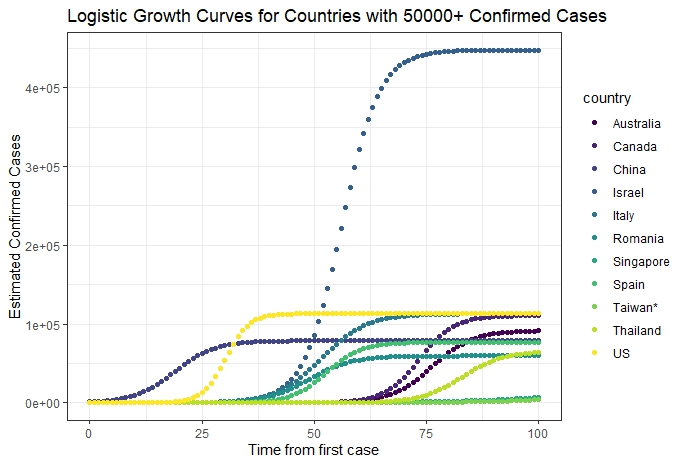
\includegraphics{./growth_curves1} \end{center}

\emph{Figure 2.}

\begin{center}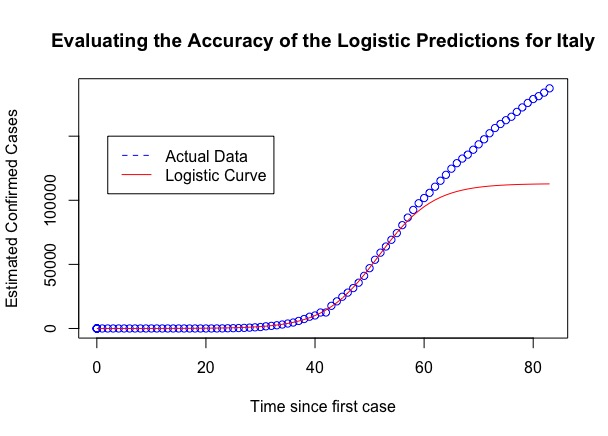
\includegraphics{./italy_predicted_cases} \end{center}

\emph{Figure 3.}

\begin{center}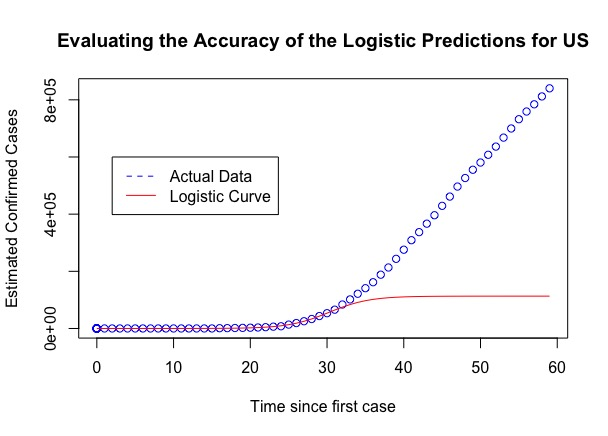
\includegraphics{./us_predicted_cases} \end{center}

\emph{Figure 4.}

\begin{center}\includegraphics{./israel_predicted_cases} \end{center}

\emph{Figure 5.}

\begin{center}\includegraphics{./togo_predicted_cases} \end{center}

\emph{Figure 6.}

\begin{center}\includegraphics{./nepal_predicted_cases} \end{center}

\emph{Figure 7. k = 4 clusters scatter plots for three parameters}

\begin{center}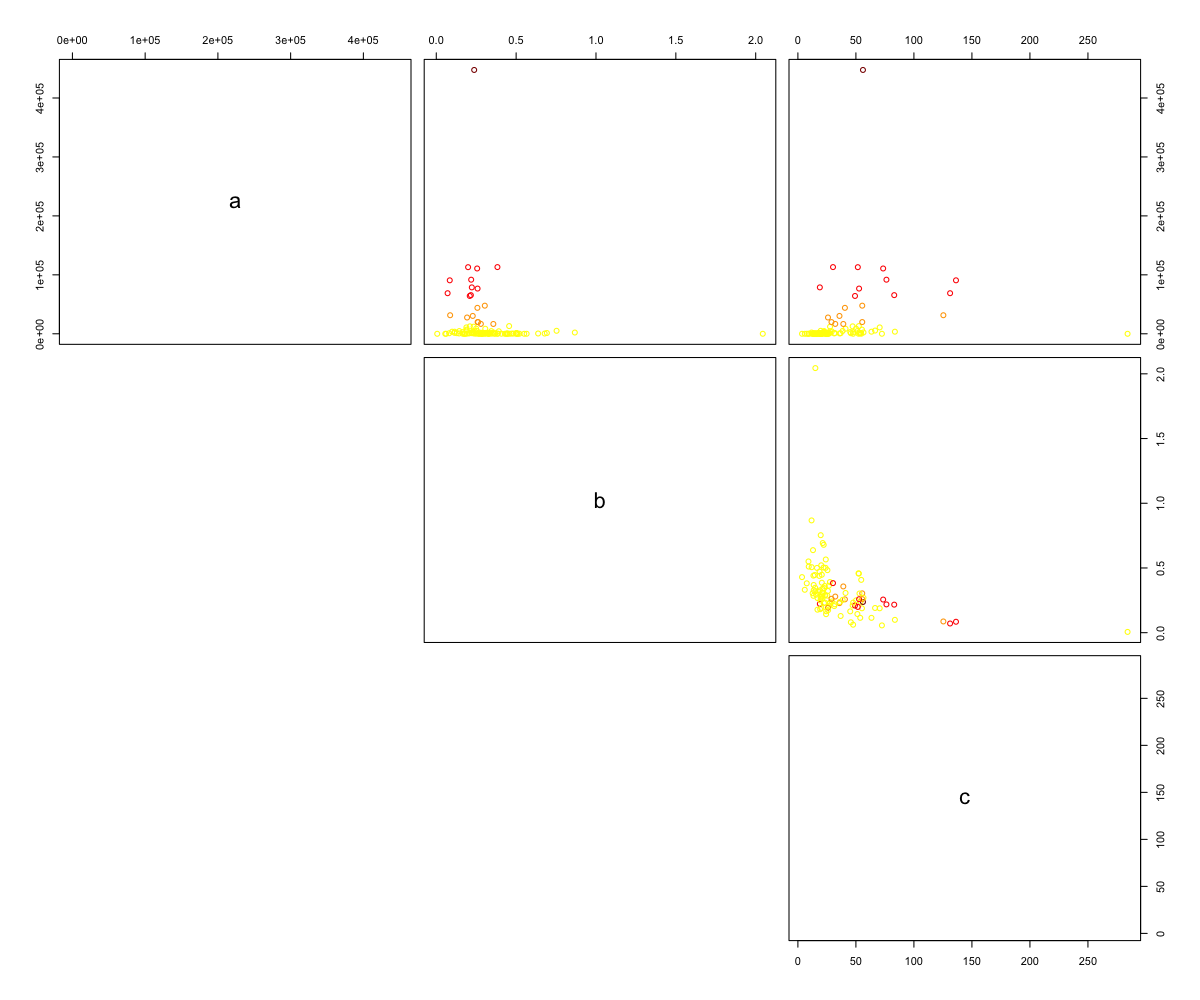
\includegraphics[width=0.5\linewidth]{./kmeans_plot} \end{center}

\emph{Figure 8.}

\begin{center}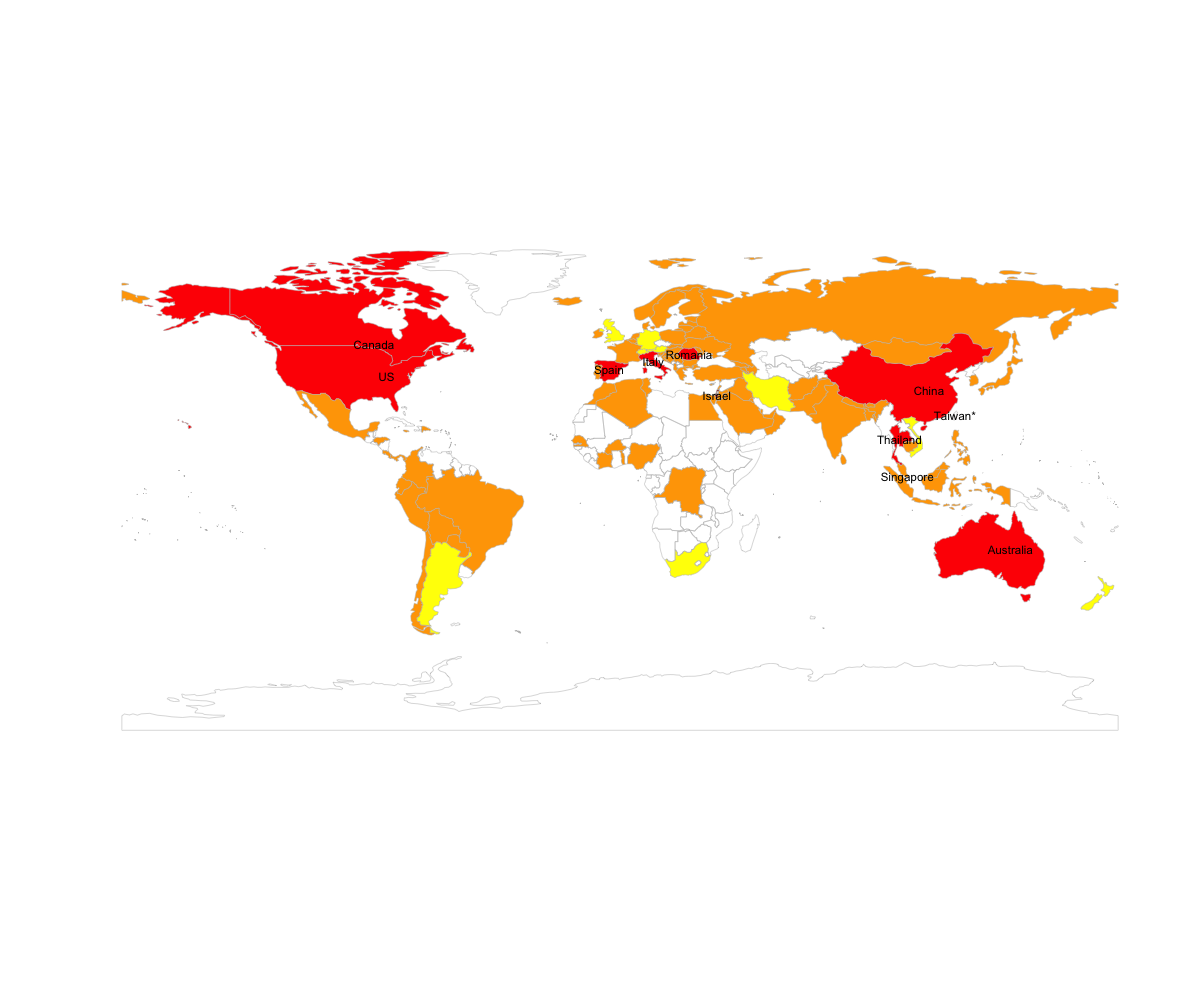
\includegraphics[width=0.9\linewidth]{./gkmeans_map} \end{center}

\emph{Figure 9.}

\begin{center}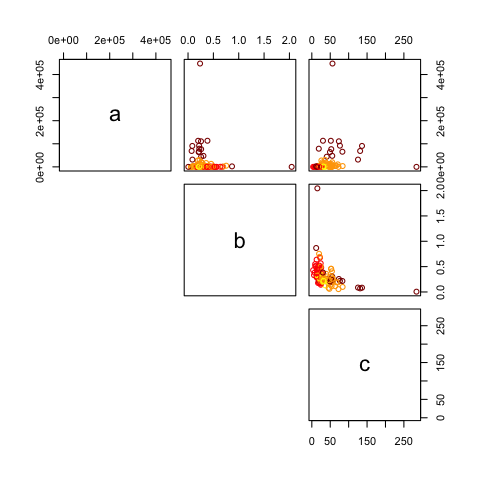
\includegraphics[width=0.9\linewidth]{./gmm_plot} \end{center}

\emph{Figure 10.}

\begin{center}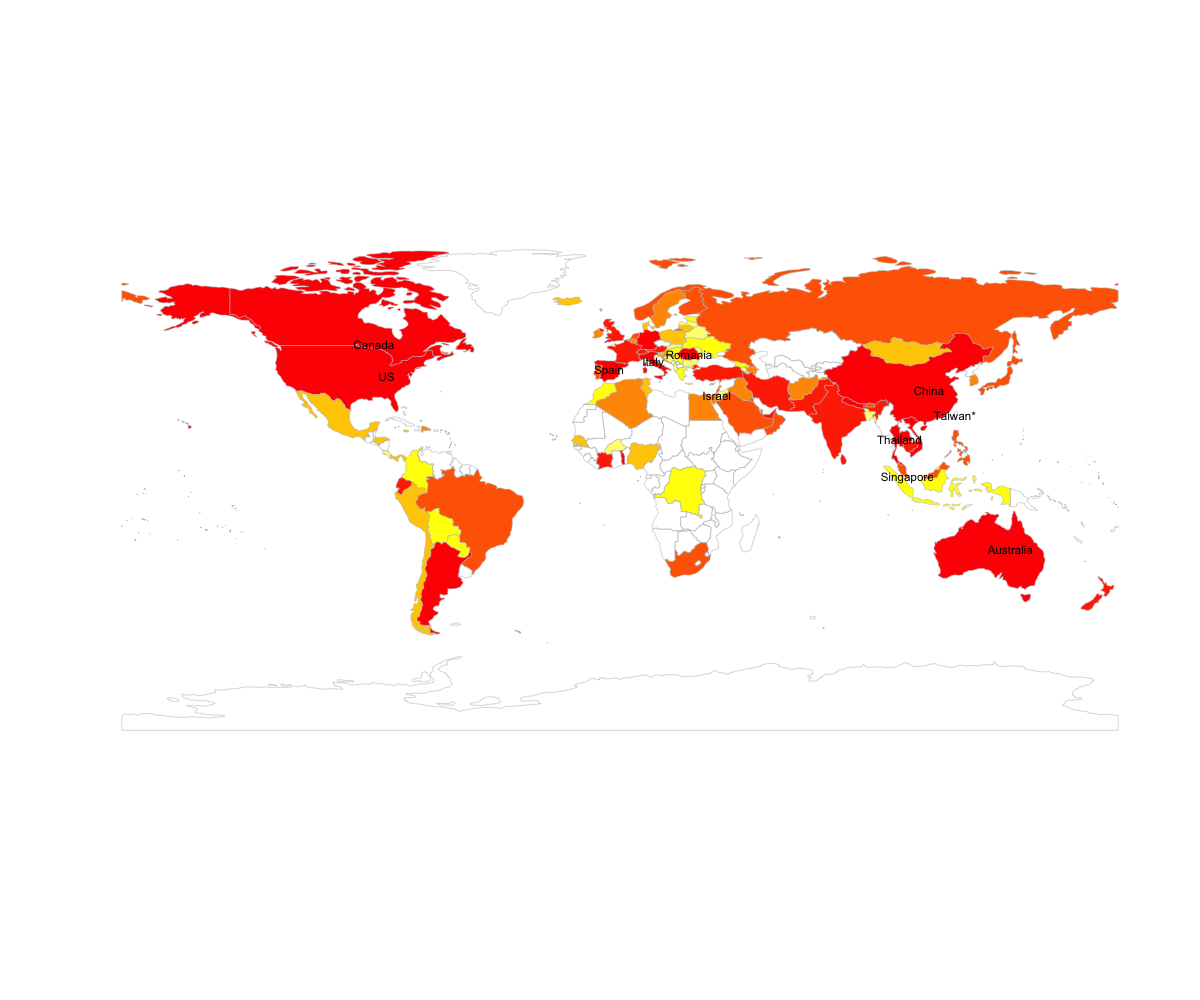
\includegraphics[width=0.9\linewidth]{./gmm_map} \end{center}

\end{document}
